\chapter{Experimental Results}
\label{chap:experimental-results}

In this chapter, we evaluate and compare the synthesizers presented in
Chapter~\ref{chap:synthesis}.
The synthesizers are compared in terms of their running time and number of
problems solved.
A description of the benchmarks is provided in Section~\ref{sec:bench-desc}.
Section~\ref{sec:results} presents the experimental evaluation of the
experiments and a comparison between the setwise synthesizer
(Section~\ref{sec:setwise-encoding}) and the whole synthesizer
(Section~\ref{sec:whole-encoding}).

\section{Benchmark Description}
\label{sec:bench-desc}

A set of 285,522 expressions were provided by OutSystems.
We conducted an analysis to determine which builtin functions and combinations
of functions were the most common in that set.
We picked 51 expressions containing only functions from
Table~\ref{table:builtin-description}, with sizes (number of components) ranging
from 1 to 7.
The size distribution of these 51 expressions is shown in
Figure~\ref{fig:bar-chart-sizes-51}.
Figure~\ref{fig:bar-chart-components-freq-51} shows the number of expressions in
which each component occurs.

\begin{figure}
  \centering
  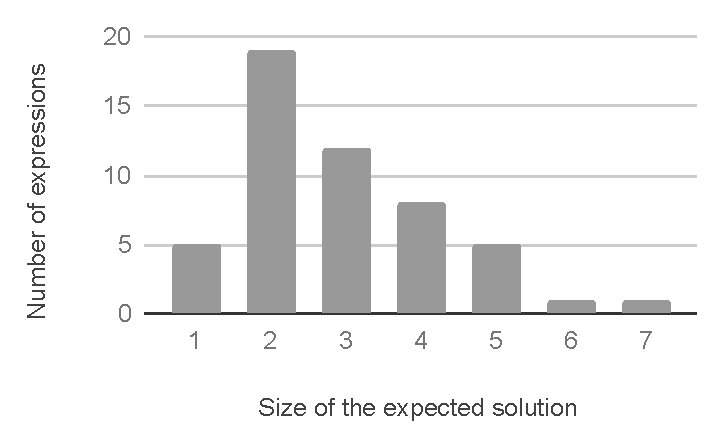
\includegraphics[width=0.5\textwidth]{assets/bar-chart-sizes-51.pdf}
  % \begin{tikzpicture}
  %   \begin{axis}[
  %     x tick label style={/pgf/number format/1000 sep=},
  %     %
  %     xlabel=Size of the intended solution,
  %     ylabel=Number of expressions,
  %     %
  %     enlargelimits=0.05,
  %     legend style={
  %       at={(0.5,-0.1)},
  %       anchor=north,
  %       legend columns=-1},
  %     ybar interval=0.7,
  %     ]
  %     % 
  %     \addplot 
  %     coordinates {
  %       (1,5)
  %       (2,19)
  %       (3,12)
  %       (4,8)
  %       (5,5)
  %       (6,1)
  %       (7,1)
  %     };
  %   \end{axis}
  % \end{tikzpicture}

  \caption{Number of expressions per size, out of 51 expressions.
    For example, there are 31 expressions of size 2, and 16 expressions of size
    1.
    Most expressions have size between 2 and 4.}
  \label{fig:bar-chart-sizes-51}
\end{figure}

The hardness of a benchmark may depend on the size of the solution, the number
of input-output examples, and the library of components.
Typically, the higher the size of the intended solution and the number of
components in the library, the harder it is to synthesize a program.

\begin{figure}
  \centering
  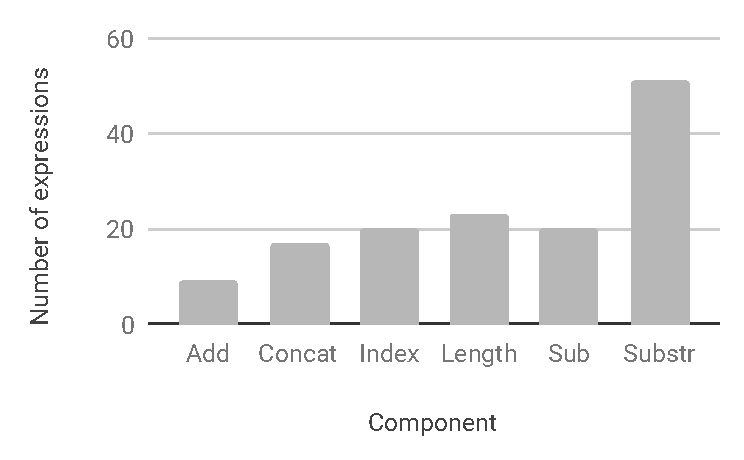
\includegraphics[width=0.5\textwidth]{assets/bar-chart-components-freq-51.pdf}
  \caption{Number of expressions per component.}
  \label{fig:bar-chart-components-freq-51}
\end{figure}

We obtained a set of 3 input-output examples for each of these 51 expressions.
In order to do that, we developed an \textit{interpreter} for OutSystems
expressions, and manually created a set of 3 different inputs for each
expression.
The inputs were carefully crafted in order to try to eliminate as much ambiguity
as possible.
Then we interpreted the expressions over their set of inputs in order to
obtain the corresponding outputs.
A first approach was tried where we encoded the expressions in \gls{smt} in such
a way that a solution to the formulas yielded valid input-output examples.
Although the approach worked, it was ultimately too slow, and the automatically
generated examples were not natural.
As a result, we resorted to the manual approach.

The \gls{smt} solver used to solve the formulas generated in the synthesis
process was Microsoft's Z3 solver~\cite{DeMoura:2008:ZES} (version 4.8.5).
Each benchmark was monitored by the \textit{runsolver}
tool~\cite{Roussel:2011:JSAT}, typically used in
SAT\footnote{\url{http://satcompetition.org/}},
MaxSAT\footnote{\url{http://www.maxsat.udl.cat}} and
PB\footnote{\url{http://www.cril.univ-artois.fr/PB16/}}
competitions, and restricted to a wall-clock time limit of 600 seconds and a
memory limit of 16 GB.
We ran the experiments in an computer with Intel(R) Xeon(R) CPU E5-2620 v4 @
2.10GHz processors running Ubuntu 16.04.5 LTS.

\section{Evaluation}
\label{sec:results}

We are interested in evaluating the impact of the number and quality of the
input-output examples on the performance of the synthesizer in terms of runtime
and program quality.
In this section, we only study the impact of the number of input-output
examples.

We present the results for both synthesizers described in
Chapter~\ref{chap:synthesis} with the following configurations.
For each instance with 3 input-output examples we ran both synthesizers using 1,
2, or 3 of the input-output examples.
We ran the setwise synthesizer (Section~\ref{sec:setwise-encoding}) configured
to synthesize programs with a maximum of one integer and one string constants
(we refer to these configurations as S-e1:c1, S-e2:c1, and S-e3:c1, for 1, 2,
and 3 input-output examples, respectively), and also with a maximum of two
integer and two string constants (configurations S-e1:c2, S-e2:c2, and S-e3:c2).
We ran the whole synthesizer (Section~\ref{sec:whole-encoding}) configured to
synthesize programs with a maximum of one constant. The synthesizer can
choose whether this constant is an integer or a string (configurations W-e1:c1,
W-e2:c1, and W-e3:c1, for 1, 2, and 3 input-output examples, respectively).
Similarly, we also run the whole synthesizer configured to use a maximum of four
constants (configurations W-e1:c4, W-e2:c4, and W-e3:c4).

In addition, we also instantiated SyPet~\cite{Feng:2017:CSC}, a
\gls{pbe} component-based synthesizer for Java programs that employs a
type-directed search together with a constraint-based technique, with our
library of components.
However, SyPet does not support guessing the value of constants.
With this in mind, we set up two configurations for SyPet.
For the first configuration (SyPet-All), we introduced a new 0-arity component
for each constant in a pool of predefined constants.\footnote{The pool of
constants, 43 in total, is the following: \lstinline{0, 1, 2, 3, 4, 5, 6, 7, 8,
9, 10, 15, 16, 20, 30, 40, 50, 60, 70, 80, 90, 100, "", "...", "/", "\", " ",
"-", ".", "@", "," "_","#","(",")","|","<",">",":","Created on ", "updated on",
"\\", " At:"}. These were chosen in order to roughly match those found in the
expected solutions. The expected solutions employ a total of 34 constants from
this pool.}
For the second configuration (SyPet-User), we looked at each particular
instance, and introduced new components only for the constants that appear in
the expected solution.
This mimics a setting where the constants are declared by the user, instead of
being guessed by the synthesizer.
Both Sypet\nobreakdash-User and Sypet-All were configured for using the three
input-output examples of each benchmark, and may use as many constants as they
need (out of the available ones).
Table~\ref{table:comparison-configs} shows a comparison between the different
configurations in terms of the number of instances solved and running wall-clock
time (mean and median for solved instances).
An instance is considered solved if the synthesized program satisfies the
input-output examples (but might or might not be what the user intended).
Matching the expected solution means, that the synthesizer outputs a program
that, not only satisfies the input-output examples, but also captures the
original intent and generalizes to more examples (this is checked by manual
inspection).
Figures~\ref{fig:bar-chart-solved-setwise-c1}
and~\ref{fig:bar-chart-solved-setwise-c2} show the number of solved instances
per size of the expected solution for the configurations S-e1:c1, S-e2:c1 and
S-e3:c1, and for configurations S-e1:c4, S-e2:c4 and S-e3:c4, respectively.
Figures~\ref{fig:bar-chart-solved-whole-c1}
and~\ref{fig:bar-chart-solved-whole-c4} show the same for configurations
W-e1:c1, W-e2:c1 and W-e3:c1, and for configurations W-e1:c4, W-e2:c4 and
W-e3:c4, respectively.
Figures~\ref{fig:bar-chart-expected-setwise-c1}
and~\ref{fig:bar-chart-expected-setwise-c2} show the number of solved instances
matching the expected solution per size of the expected solution for
configurations S-e1:c1, S-e2:c1 and S-e3:c1, and for configurations
S-e1:c4, S-e2:c4 and S-e3:c4, respectively.
Figures~\ref{fig:bar-chart-solved-whole-c1}
and~\ref{fig:bar-chart-expected-whole-c4} show the same for configurations
W-e1:c1, W-e2:c1 and W-e3:c1, and for configurations W-e1:c4, W-e2:c4 and
W-e3:c4, respectively.
Figures~\ref{fig:comparison-solved-sypet} and
\ref{fig:comparison-expected-sypet} show a comparison between all configurations
on three input-output examples.

\section{Discussion}
\label{sec:discussion}

The sizes of both encodings grow linearly with the number of input-output
examples. Indeed, we can verify that the hardness of the problem increases with
the number of examples (Figures~\ref{fig:bar-chart-solved-setwise-c1},
\ref{fig:bar-chart-solved-setwise-c2}, \ref{fig:bar-chart-solved-whole-c4}
and~\ref{fig:bar-chart-solved-whole-c4}).
This effect becomes more significant as we increase the size of the expected
solution.
On the other hand, the number of programs matching the expected solution should
increase with the number of input-output examples, which we can also verify from
the results in Figures~\ref{fig:bar-chart-expected-setwise-c1},
\ref{fig:bar-chart-expected-setwise-c2}, \ref{fig:bar-chart-expected-whole-c4}
and~\ref{fig:bar-chart-expected-whole-c4}.
In Figures~\ref{fig:comparison-solved-sypet}
and~\ref{fig:comparison-expected-sypet} we can see that SyPet-All has similar
results to the whole synthesizer.
The large number of components makes the search space intractable.
Besides, it cannot take advantage of its type-directed algorithm because we are
dealing with only two types (integers and strings).
This last point also applies to SyPet-User, but the advantage given by the
user-provided constants proves crucial for its fairly good results, which are
actually better than the ones obtained for the setwise synthesizer
(Table~\ref{table:comparison-configs}).
However, recall that the setwise synthesizer is solving a harder problem because
it computes the constants itself.

Many expected solutions require more than one constant, with some requiring more
than one constant of each type.
This could lead one to think that that is the origin of the poor performance of
the whole encoding.
However, we can see that increasing the number of available constants leads to
even worse results in both synthesizers (on these instances).
The configurations with more constants available lead to more instances solved
and in less time, but also lead to less intended solutions.
It could also be speculated from the start that the whole synthesizer would
perform worse than the setwise synthesizer.
Typically, one would expect that solving one large constraint is more expensive
than solving multiple smaller constraints.\footnote{Note that the \gls{smt}
problem with the theory of strings and linear arithmetic is undecidable.}

The running times for the solved benchmarks are reasonably fast, allowing for
tolerable interaction times with the user.
However, synthesizing programs with 4 or more lines seems to be out of reach for
these configurations (Figure~\ref{fig:comparison-expected-sypet}).

\begin{table}[]
  \noindent\makebox[\textwidth]{
    \begin{tabular}{ccccc}
      \toprule

      \multicolumn{1}{l}{Configuration}
      & \multicolumn{1}{l}{\# Instances solved}
      & \begin{tabular}[c]{@{}c@{}}\# Instances solved\\ (matching expected\\ solution)\end{tabular}
      & Mean Time (s)
      & \multicolumn{1}{l}{Median Time (s)}
      \\ \midrule

      S-e1:c1    & 48 & 3  & 4.62  & 0.48 \\ \midrule 
      S-e1:c2    & 49 & 6  & 0.67  & 0.29 \\ \midrule 
      S-e2:c1    & 39 & 21 & 51.28 & 3.21 \\ \midrule
      S-e2:c2    & 42 & 13 & 46.30 & 1.12 \\ \midrule
      S-e3:c1    & 34 & 23 & 51.38 & 4.47 \\ \midrule
      S-e3:c2    & 34 & 19 & 39.97 & 1.34 \\ \midrule
      W-e1:c1    & 47 & 2  & 6.76  & 0.65 \\ \midrule
      W-e1:c4    & 50 & 4  & 2.69  & 0.09 \\ \midrule
      W-e2:c1    & 13 & 4  & 11.14 & 2.24 \\ \midrule
      W-e2:c4    & 17 & 7  & 50.37 & 0.15 \\ \midrule
      W-e3:c1    & 9  & 5  & 21.45 & 7.48 \\ \midrule
      W-e3:c4    & 10 & 5  & 0.27  & 0.17 \\ \midrule
      SyPet-All  & 11 & 6  & 31.27 & 3.00 \\ \midrule
      SyPet-User & 32 & 30 & 52.75 & 5.00 \\ \bottomrule

    \end{tabular}}
  \caption{Comparison between the different configurations by number of instances
    solved and running wall-clock time for solved instances (not necessarily
    matching the expected solution).}
  \label{table:comparison-configs}
\end{table}

% Solved setwise
\begin{figure}
  \centering
  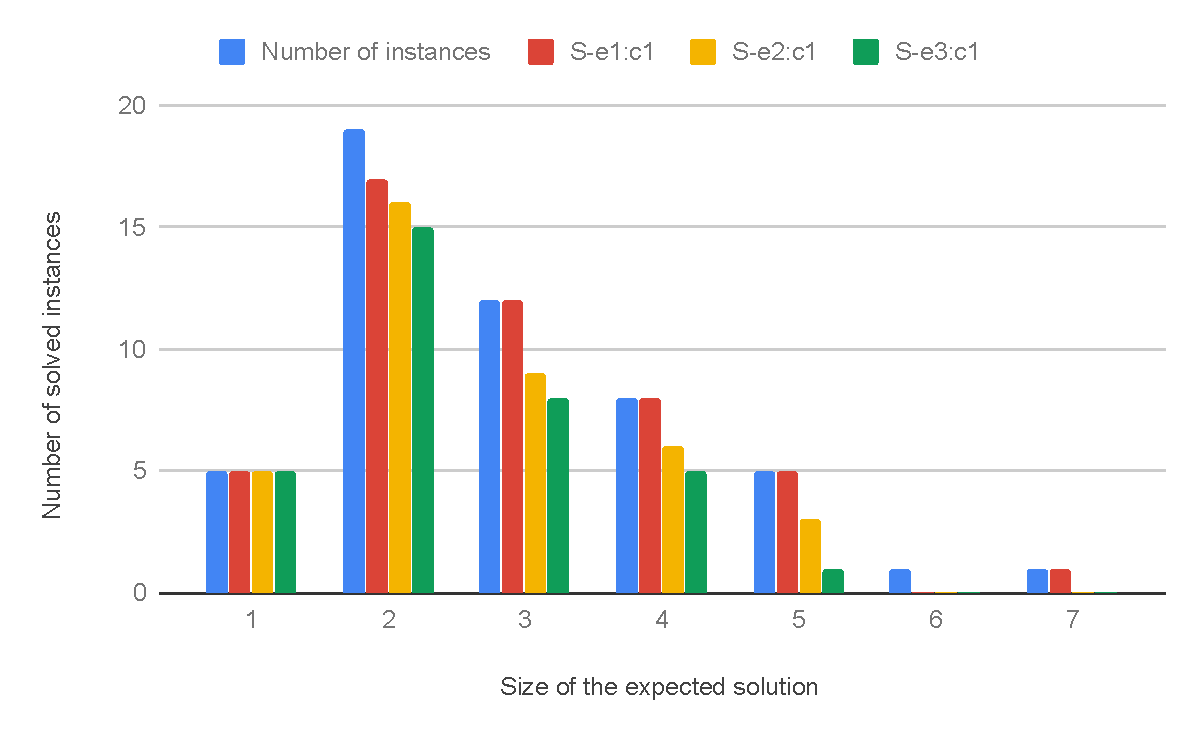
\includegraphics[width=1.0\textwidth]{assets/bar-chart-solved-setwise-c1.pdf}
  \caption{Number of solved instances per size of the expected solution for
    the setwise synthesizer with one, two, and three examples, one integer
    constant, and one string constant (S-e1:c1, S-e2:c1, S-e3:c1, respectively).}
  \label{fig:bar-chart-solved-setwise-c1}
\end{figure}

\begin{figure}
  \centering
  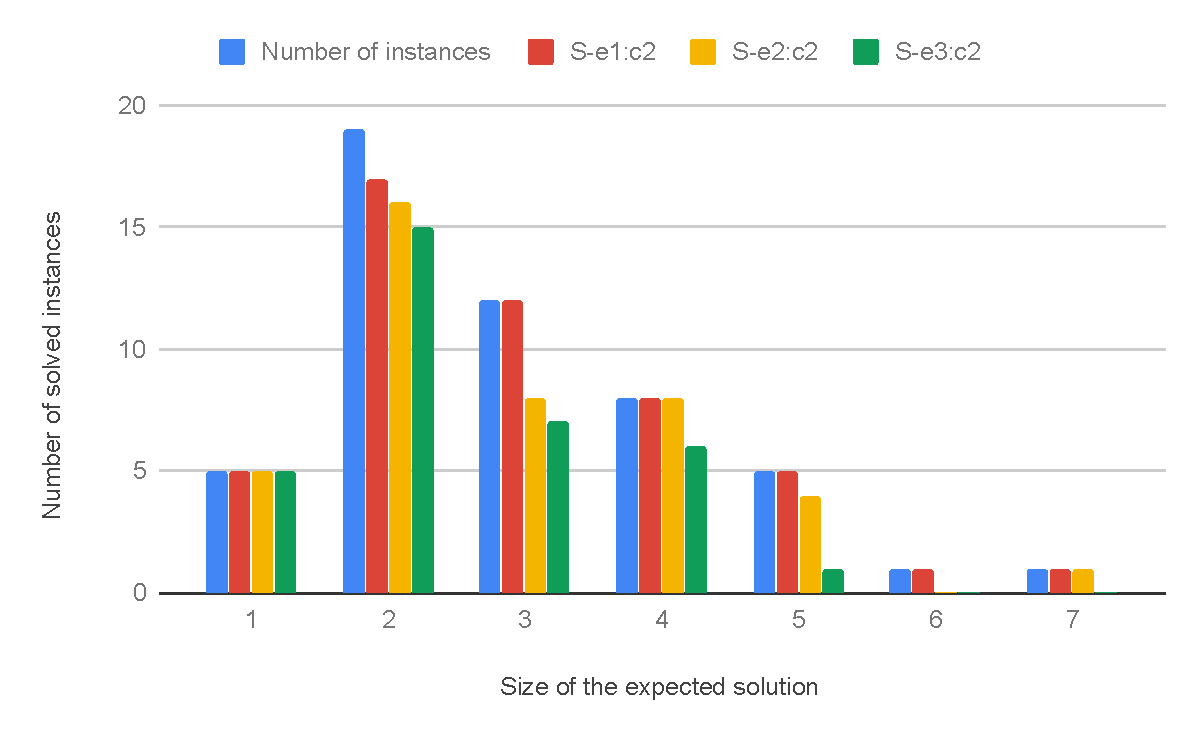
\includegraphics[width=1.0\textwidth]{assets/bar-chart-solved-setwise-c2.pdf}
  \caption{Number of solved instances per size of the expected solution for
    the setwise synthesizer with one, two, and three examples, two integer
    constants, and two string constants (S-e1:c2, S-e2:c2, S-e3:c2,
    respectively).}
  \label{fig:bar-chart-solved-setwise-c2}
\end{figure}

% Solved whole
\begin{figure}
  \centering
  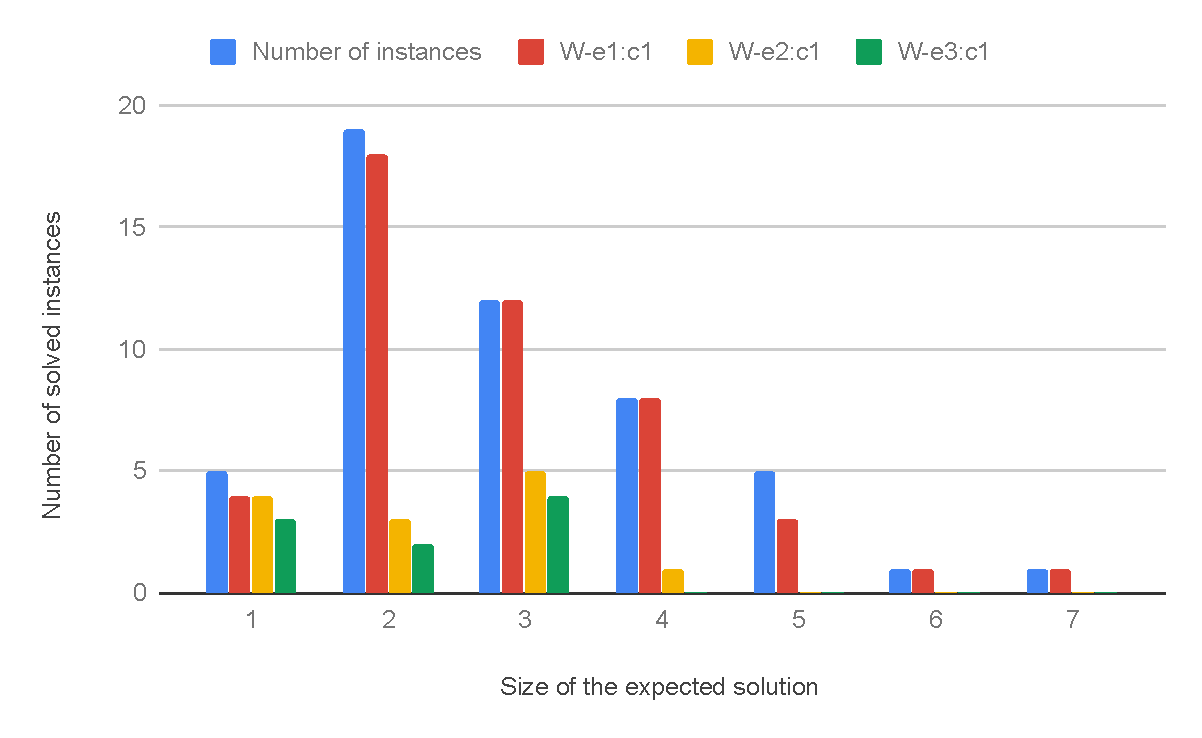
\includegraphics[width=1.0\textwidth]{assets/bar-chart-solved-whole-c1.pdf}
  \caption{Number of solved instances per size of the expected solution for
    the whole synthesizer with one, two, and three examples, and one constant
    (W-e1:c1, W-e2:c1, W-e3:c1, respectively).}
  \label{fig:bar-chart-solved-whole-c1}
\end{figure}

\begin{figure}
  \centering
  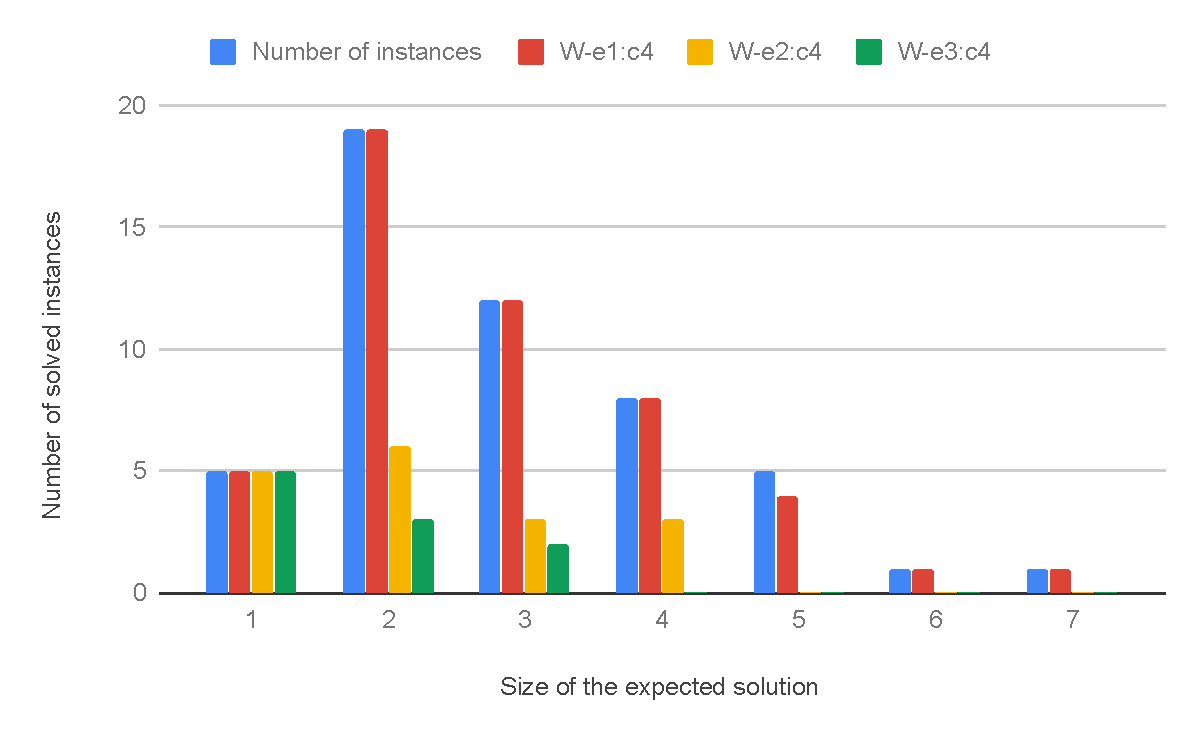
\includegraphics[width=1.0\textwidth]{assets/bar-chart-solved-whole-c4.pdf}
  \caption{Number of solved instances per size of the expected solution for
    the whole synthesizer with one, two, and three examples, and four constants
    (W-e1:c4, W-e2:c4, W-e3:c4, respectively).}
  \label{fig:bar-chart-solved-whole-c4}
\end{figure}

% Expected setwise
\begin{figure}
  \centering
  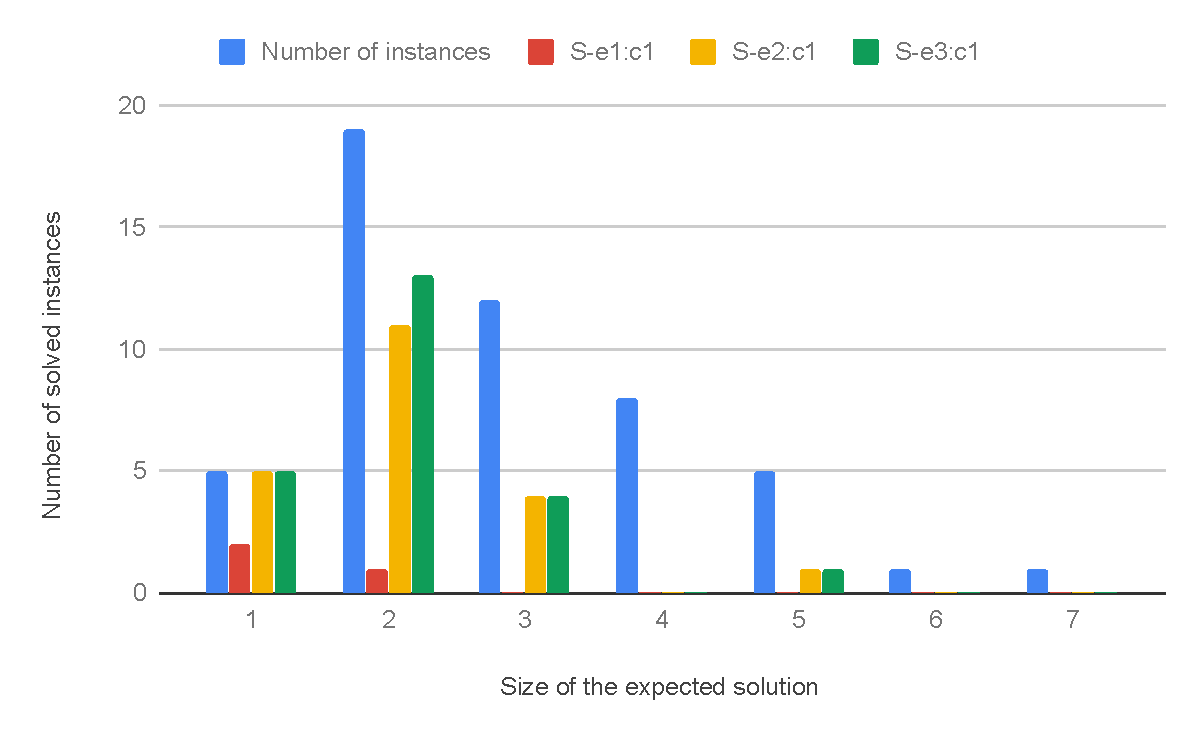
\includegraphics[width=1.0\textwidth]{assets/bar-chart-expected-setwise-c1.pdf}
  \caption{Number of solved instances matching the expected solution per size of
    the expected solution for the setwise synthesizer with one, two, and three
    examples, one integer constant, and one string constant (S-e1:c1, S-e2:c1,
    S-e3:c1, respectively).}
  \label{fig:bar-chart-expected-setwise-c1}
\end{figure}

\begin{figure}
  \centering
  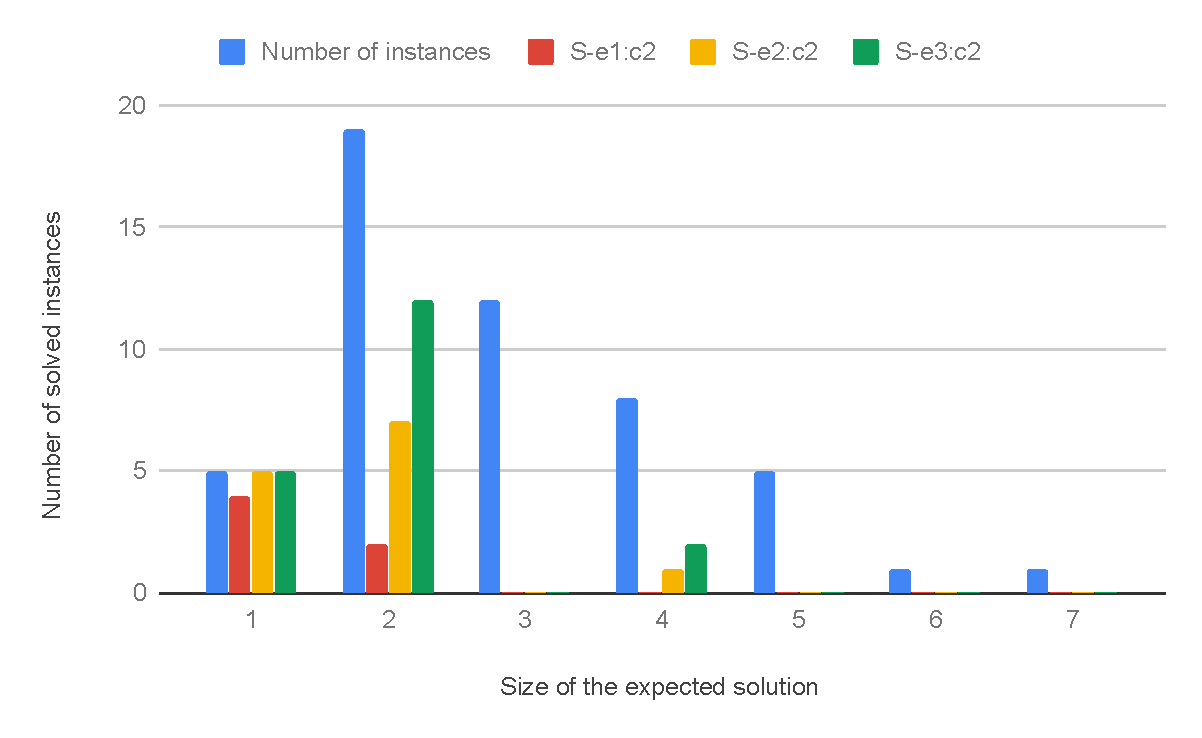
\includegraphics[width=1.0\textwidth]{assets/bar-chart-expected-setwise-c2.pdf}
  \caption{Number of solved instances matching the expected solution per size of
    the expected solution for the setwise synthesizer with one, two, and three
    examples, two integer constants, and two string constants (S-e1:c2, S-e2:c2,
    S-e3:c2, respectively).}
  \label{fig:bar-chart-expected-setwise-c2}
\end{figure}

% Expected whole
\begin{figure}
  \centering
  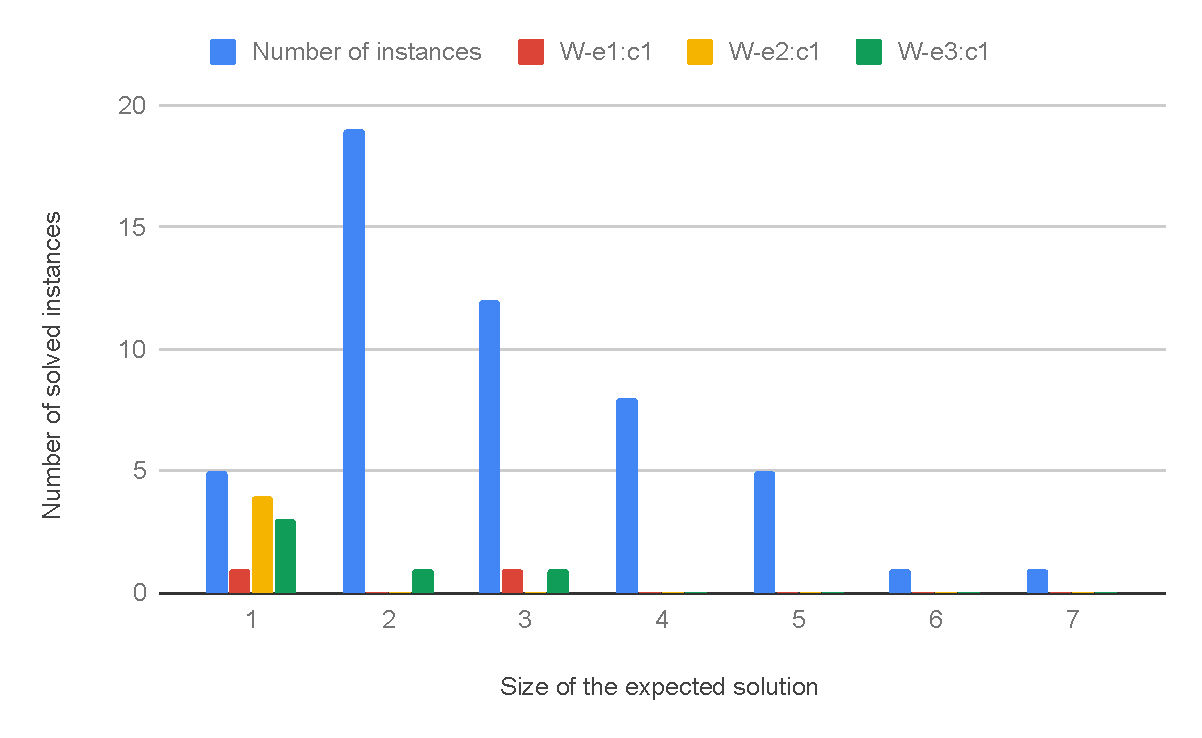
\includegraphics[width=1.0\textwidth]{assets/bar-chart-expected-whole-c1.pdf}
  \caption{Number of solved instances matching the expected solution per size of
    the expected solution for the whole synthesizer with one, two, and three
    examples, and one constant (W-e1:c1, W-e2:c1, W-e3:c1, respectively).}
  \label{fig:bar-chart-expected-whole-c1}
\end{figure}

\begin{figure}
  \centering
  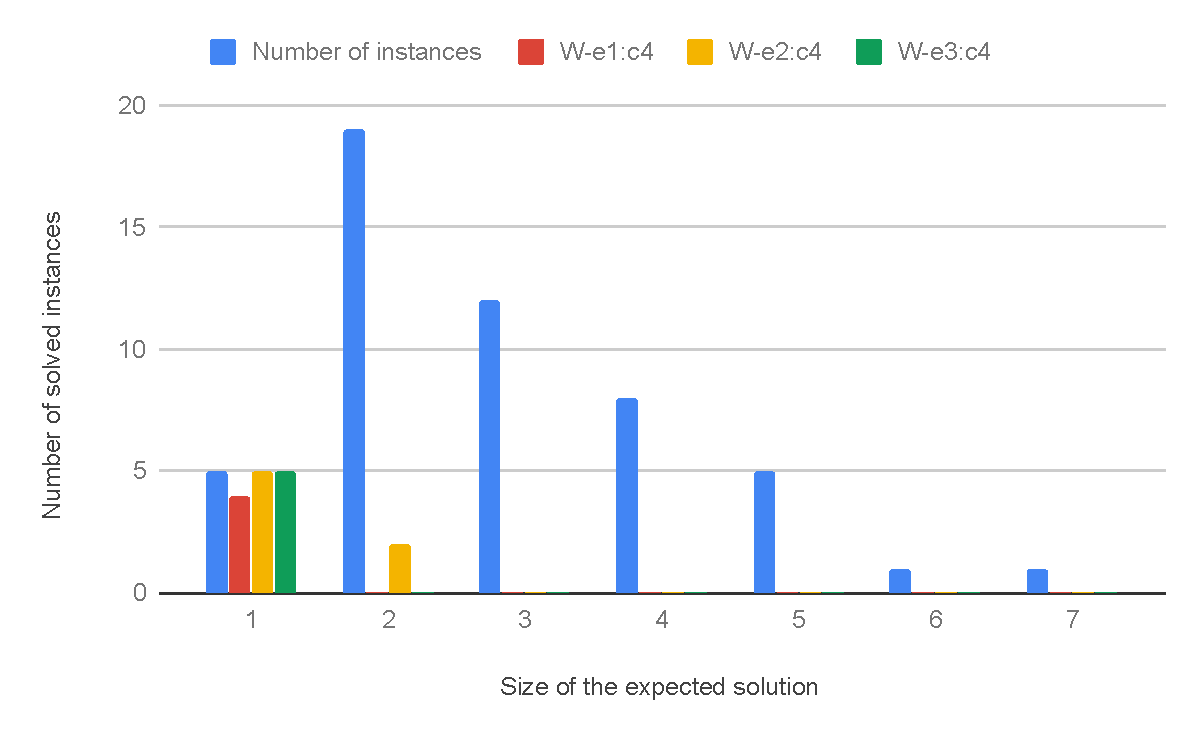
\includegraphics[width=1.0\textwidth]{assets/bar-chart-expected-whole-c4.pdf}
  \caption{Number of solved instances matching the expected solution per size of
    the expected solution for the whole synthesizer with one, two, and three
    examples, and four constants (W-e1:c4, W-e2:c4, W-e3:c4, respectively).}
  \label{fig:bar-chart-expected-whole-c4}
\end{figure}

% Solved comparison
\begin{figure}
  \centering
  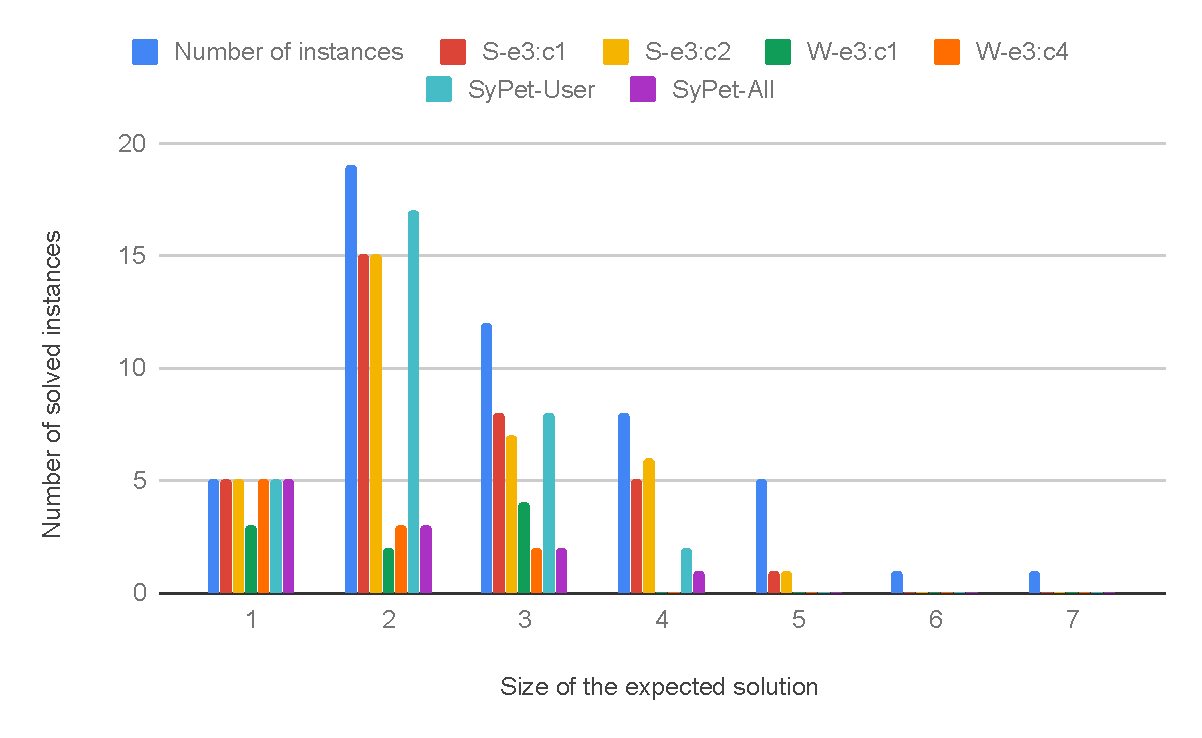
\includegraphics[width=1.0\textwidth]{assets/comparison-solved-sypet-new.pdf}
  \caption{Number of solved instances per size of the expected solution for the
    setwise and whole synthesizers with three examples, and both SyPet
    configurations.}
  \label{fig:comparison-solved-sypet}
\end{figure}

% Expected comparison
\begin{figure}
  \centering
  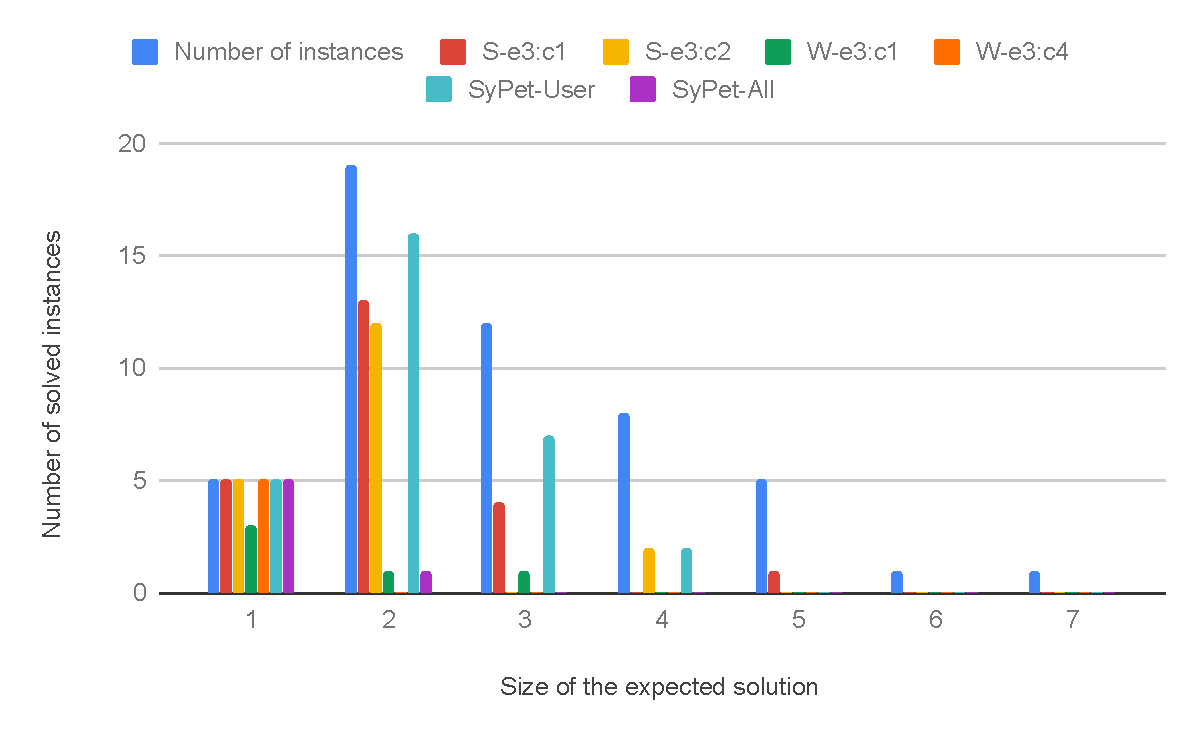
\includegraphics[width=1.0\textwidth]{assets/comparison-expected-sypet-new.pdf}
  \caption{Number of solved instances matching the expected solution per size of
    the expected solution for the setwise and whole synthesizers with three
    examples, and both SyPet configurations.}
  \label{fig:comparison-expected-sypet}
\end{figure}
